\chapter{El Sistema de Televisión Digital Terrestre ISDB-T}

El esquema de transmisión del estándar ISDB-T que se presenta en la Figura \ref{f:esquema-tx} puede ser caracterizado en cuatro grandes etapas que serán presentadas en este capítulo: el flujo de transporte BTS (\textit{Broadcast Transport Stream}), la etapa de robustecimiento de la señal, la formación de los Cuadros OFDM con sus señales piloto y la puesta en el aire de la señal.

Cada una de esas etapas tiene a su vez varias subetapas, o bloques fundamentales, que se enfocan en resolver los distintos problemas discutidos que surgen al transmitir una señal inalámbrica. Esto dá como resultado una variedad de parámetros de operación presentados en la Tabla \ref{parametros_ISDBT} que permitirán por ejemplo, la transmisión jerárquica en distintas capas, cada una con su propia configuración; o enfocarse en robustecer la transmisión frente al \textit{multipath} o al efecto Doppler.

A nivel de la distribuci\'on en el espectro, el estándar utiliza 6 MHz de ancho de banda de canal distribu\'ido en 14 segmentos de los cuales sólo 13 son utilizados para enviar datos, el restante se utiliza como guarda a ambos lados del canal. Tambi\'en se incluye un piloto continuo que se trata de una portadora modulada en BPSK ubicada a continuaci\'on del Segmento 12.

\begin{figure}
\centering
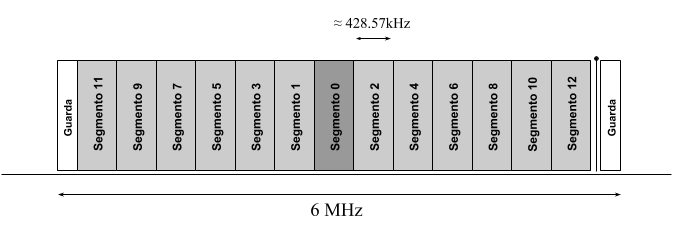
\includegraphics[scale=0.55]{figuras/cap03/segmentos_isdbt}
\caption{\label{segmentos_isdbt} Distribuci\'on espectral de los segmentos OFDM. A la derecha puede apreciarse la presencia del piloto continuo.}
\end{figure}

Tener un esquema de transmisi\'on jer\'arquica permite asignar a cada capa jer\'arquica la cantidad de segmentos que uno quiera. El est\'andar de la ARIB denomina a estas capas como A, B y C, y es posible tener configurac\'ones con solamente 2 capas presentes tal como la de la Figura \ref{segmentos_isdbt} en la que la capa A corresponde al segmento 0 y el resto de los segmentos forman la capa B.

En los comienzos de la televisi\'on digital en el Uruguay los operadores que prestaban servicios de televisi\'on digital deb\'ian transmitir su señal en calidad HD, en SD y \textit{oneseg}, es decir en tres capas jer\'arquicas. Esto era as\'i porque se entend\'ia que en el mercado circulaba una gran cantidad de receptores que no eran capaces de procesar la calidad HD. Posteriormente esa directiva fu\'e suprimida y al d\'ia de hoy los operadores no est\'an obligados a transmitir en SD.

El sistema puede operar en tres \textit{modos de transmisi\'on} diferentes que se caracterizan por la cantidad de portadoras utilizadas, siempre en el mismo ancho de banda de 6 MHz. Las portadoras utilizadas son $2^{10+modo}$ donde el modo puede ser 1, 2 o 3.

Se define la frecuencia de muestreo de la IFFT como $f_{IFFT} \triangleq \frac{512}{63 \mu s} \approx 8.127 MHz$, que a su vez coincide con el n\'umero de portadoras utilizadas sobre el tiempo de s\'imbolo activo $T_s$. Por lo tanto la utilizaci\'on de un n\'umero mayor de portadoras implica utilizar s\'imbolos m\'as largos para respetar la relaci\'on de la $f_{IFFT}$; aumentar el tiempo de s\'imbolo activo implica reducir el ancho de banda ocupado por cada portadora.

Cada segmento a su vez est\'a conformado por dos tipos de señales portadoras. Las primeras son las correspondientes a los datos, y las otras son las denominadas \textit{portadoras piloto} que cumplen se utilizan para la estimaci\'on del canal y transmisi\'on de par\'ametros de control e informaci\'on del sistema.
De manera general, los segmentos tienen $96 \times 2^{modo-1}$ portadoras de datos $12 \times 2^{modo-1}$ portadoras piloto dependiendo del modo de transmisi\'on. En la Tabla \ref{parametros_ISDBT} se eval\'uan estos par\'ametros para los distintos modos de transmisi\'on. 

******* Prefijo c\'iclico (Considerar lo que se hablo en el CAP 2 para no ser reiterativos)******.

\begin{figure}
\centering
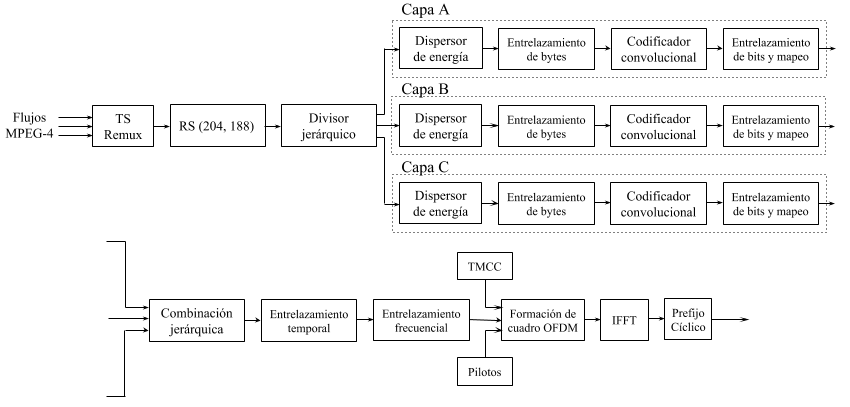
\includegraphics[scale=0.55]{figuras/cap03/esquema-tx}
\caption{\label{f:esquema-tx} Diagrama de bloques del transmisor ISDB-T definido por la ARIB.}
\end{figure}


\begin{table}[h!]
\centering
\begin{tabular}{|c|c|}
\hline
\textbf{Parámetro} 				& \textbf{Valor}\\
\hline
Ancho de banda del canal 		& 6 MHz\\
\hline
Cantidad de segmentos 			& 13 \\
\hline
Ancho de banda de cada segmento & $6000/14 \approx 428.57kHz$ \\
\hline
  											& 96 de datos y 12 pilotos (Modo 1) \\
Cantidad de portadoras activas por segmento & 192 de datos y 24 pilotos (Modo 2) \\
 											& 384 de datos y 48 pilotos (Modo 3)\\
\hline
 								& $252 \mu s$ (Modo 1)\\
Duración de símbolo activo 		& $504 \mu s$ (Modo 2) \\
								& $1008 \mu s$ (Modo 3) \\
\hline
Duracion del prefijo ciclico 	& 1/4, 1/8, 1/16, 1/32 \\
 								& (fraccion del simbolo activo)\\
\hline
Tasa de codigo convolucional 	& 1/2, 2/3, 3/4, 5/6, 7/8\\
\hline
Tasa de codigo Reed-Solomon 	& (188, 204) \\
\hline
 								& 0, 1, 2, 4 (Modo 1) \\
Profundidad del entrelazamiento temporal & 0, 2, 4, 8 (Modo 2) \\
 & 0, 4, 8, 16 (Modo 3)\\
\hline
Esquemas de modulacion & DQPSK, QPSK,\\
 & 16QAM, 64QAM\\
 \hline
 Frecuencia de muestreo ($f_{IFFT}$) & 512/63 $\approx$ 8.127 MHz\\
 \hline
\end{tabular}
\caption{\label{parametros_ISDBT} Par\'ametros relevantes en el est\'andar ISDB-T.}
\end{table}

\section{BTS como fuente de datos}

El est\'andar ISDB-T admite la posibilidad de tomar hasta tres \textit{Transport Streams} (TS) MPEG-4. A estos flujos se les debe agregar la informaci\'on necesaria para la transmisi\'on en capas jer\'arquicas. El bloque TS Remux es el que se encarga de multiplexar los tres flujos de transporte y a cada TSP agregarle 16 bytes de informaci\'on. 
Una vez que se agregan estos datos los paquetes de cada capa son multiplexados seg\'un un patr\'on de ordenamiento que es \'unico para cada configuraci\'on del sistema, en \cite{multiplex-pattern} se explica este patr\'on y se presenta un algoritmo para recuperarlo en recepci\'on. El transmisor implementado en este trabajo toma como flujo de entrada un BTS ya conformado, y con la informaci\'on jer\'arquica de los TSP es que logra procesar cada capa por separada. De ah\'i en adelante las capas son entrelazadas y moduladas cada una de acuerdo a su propia configuraci\'on. 

\section{Robustecimiento frente a las no idealidades del canal}

Como primer medida para proteger los datos del BTS se aplica un c\'odigo Reed-Solomon (204, 188). El proceso de codificaci\'on consiste en sustituir los \'ultimos 16 bytes de los TSP por una paridad que permite corregir hasta 8 bytes de error en el paquete. 

Este bloque remueve la informaci\'on jer\'arquica agregada por el TS Remux con lo cual una vez que los TSP son codificados por el Reed-Solomon en principio ya no es posible distinguir a qu\'e capa pertenece cada paquete, es decir que al llegar al bloque de divisi\'on jer\'arquica ya no se cuenta con esa informaci\'on. Una estrategia para sortear este problema, y de hecho la que se implementa en \textit{gr-isdbt-tx}, consiste en separar primero los paquetes correspondientes a cada capa jer\'arquica y luego codificar los paquetes. Una vez encaminados los paquetes se puede prescindir de la informaci\'on jer\'arquica. El diagrama de bloques presentado en la Figura \ref{f:esquema-tx} corresponde al esquema original de la ARIB en la que se define el est\'andar ISDB-T, mientras que la Figura \ref{f:esquema-tx} se encuentra la implementaci\'on utilizada en \textit{gr-isdbt-tx}. 

% Dispersor de energia
Para evitar los problemas de sincronismo que podr\'ia ocasionar una se\'al con muchos ceros o unos consecutivos, se utiliza un \textit{dispersor de energ\'ia} que se encarga de generar un flujo pseudoaleatorio. Este proceso se define de manera tal que resulta ser totalmente invertible y por lo tanto aplicando el mismo proceso en recepc\'ion se obtiene la secuencia original.



% Entrelazamiento
Los canales inal\'ambricos son propensos a una multiplicidad de fuentes de error. Un tipo de errores muy comunes en estos canales son los \textit{errores en r\'afaga} provocando que una secuencia consecutiva de bits se corrompan. El impacto de estos tipos de errores crece con la velocidad de transmisi\'on; a mayor velocidad de transmisi\'on un mismo error afecta a una mayor cantidad de bits.
Resulta necesario lograr alg\'un tipo de inmunidad ante estos errores, es por ello que en muchos sistemas, y en particular en ISDB-T, se suelen concatenar c\'odigos correctores de errores. David Forney en su trabajo \textit{Concatenated Codes} \cite{forney1965concatenated} estudia el compromiso que existe en la utilizaci\'on de sucesivos c\'odigos concatenados, y en especial la performance que pueden llegar a alcanzar los c\'odigos Reed-Solomon concatenados.
El est\'andar ISDB-T utiliza este enfoque a trav\'es de la implementaci\'on de un c\'odigo Reed-Solomon como \textit{outer code} y un c\'odigo convolucional como \textit{inner code}.
Como medida adicional para contrarrestar los efectos del canal se utiliza el \textit{entrelazamiento de bits} que esencialmente consiste en introducir retardos variables en los bits que se transmiten.

Al transmitir en m\'ultiples portadoras ortogonales se corre el riesgo de atravesar canales selectivos en frecuencia y por lo tanto que ciertas portadoras se vean continuamente afectadas. Para mitigar esto una estrategia puede ser rotar de portadora los contenidos que se transmiten, es decir hacer un \textit{entrelazamiento frecuencial}. Con esto se logra que ante un canal selectivo, ya lo sea por sus caracter\'isticas propias o por interferencias de señales espurias fuera de banda, las portadoras que son afectadas no resulte en una p\'erdida de bloques de informaci\'on irrecuperables.


\section{Las portadoras y la modulacion}


DATOS
Scattered Pilot
TMCC
AC
Piloto Continuo
\section{Formacion de los frames OFDM}
\section{La puesta en el aire de la señal}

?Equipos USRP, Antenas, ganancias, potencia, SNR necesario (??por esto es que no logramos recibir aun???)?

\begin{table}[h!]
\centering
\begin{tabular}{|c|cccc}   %center
\cline{1-4}
\textbf{Modo de transmisi\'on} & \multicolumn{1}{c|}{\textbf{Modo 1}} & \multicolumn{1}{c|}{\textbf{Modo 2}} & \multicolumn{1}{c|}{\textbf{Modo 3}} &  \\ \cline{1-4}
\textbf{Entrelazamiento de byte} 					&                   			  & 1 Cuadro 					   & \multicolumn{1}{c|}{} 			&  \\ \cline{1-4}
\textbf{Entrelazamiento de bit} 						&					   			  & 2 S\'imbolos OFDM 			   & \multicolumn{1}{c|}{} 			&  \\ \cline{1-4}
\multirow{4}{*}{\textbf{Entrelazamiento temporal}}	&\multicolumn{1}{c|}{0 Cuadros (I = 0)} & \multicolumn{1}{c|}{0 Cuadros (I = 0)} & \multicolumn{1}{c|}{0 Cuadros (I = 0)} &  \\ \cline{2-4}
  										    &\multicolumn{1}{l|}{2 Cuadros (I = 4)} & \multicolumn{1}{c|}{1 Cuadros (I = 2)} & \multicolumn{1}{c|}{1 Cuadros (I = 1)} &  \\ \cline{2-4}
											&\multicolumn{1}{c|}{4 Cuadros (I = 8)} & \multicolumn{1}{c|}{2 Cuadros (I = 4)} & \multicolumn{1}{c|}{1 Cuadros (I = 2)} &  \\ \cline{2-4}
											&\multicolumn{1}{l|}{8 Cuadros (I = 16)} & \multicolumn{1}{c|}{4 Cuadros (I = 8)} & \multicolumn{1}{c|}{2 Cuadros (I = 4)} &  \\ \cline{1-4}
\textbf{Combinaci\'on jer\'arquica}			& 				   			    & 2 Cuadros 			 & \multicolumn{1}{c|}{} 		  &  \\ \cline{1-4}
\end{tabular}
\caption{\label{delays_agregados} Retardos agregados por los bloques en transmisi\'on.}
\end{table}